\section{
    Implemente no JFlap uma Máquina de Turing que, dada uma cadeia binária com ocorrências de \#’s, remova todas essas ocorrências, independentemente de suas posições
    }

\setlength{\parindent}{4em}
\setlength{\parskip}{0.5em}
\renewcommand{\baselinestretch}{1}

\begin{figure}[h]
    \centering
    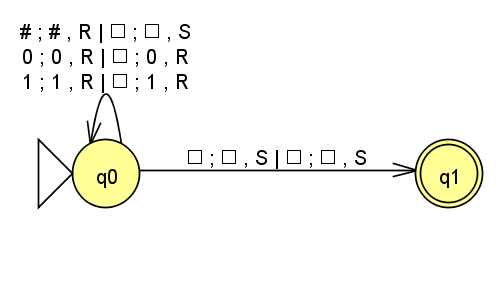
\includegraphics[width=0.65\textwidth]{mtex2.png}
    \caption{Máquina de Turing desenvolvida para o exercício no JFlap.}
    \label{fig:mtex2}
\end{figure}

A máquina de Turing desenvolvida é de fita dupla. Ela considera que a primeira fita é o input e na segunda fita escreve o output.

Ela lê a primeira fita símbolo a símbolo sequencialmente, seguindo as seguintes regras:
\begin{itemize}
    \item Caso o símbolo lido seja 1, na primeira fita ela vai reescrever esse 1 e mover a cabeça de leitura para a direita e na segunda fita, ela vai escrever o símbolo 1 e mover a cabeça de leitura para a direita.
    
    \item Caso o símbolo lido seja 0, na primeira fita ela vai reescrever esse 0 e mover a cabeça de leitura para a direita e na segunda fita, ela vai escrever o símbolo 0 e mover a cabeça de leitura para a direita.

    \item Caso o símbolo lido seja \#, na primeira fita ela vai reescrever esse \# e mover a cabeça de leitura para a direita e na segunda fita, ela não escreve nada e mantém a cabeça de leitura na mesma posição.

    \item Quando chegar ao final da fita, ela mantém ambas as cabeças de leitura na mesma posição e muda de estado para o estado final \(q1\).
\end{itemize}

O arquivo do JFlap com a implementação da Máquina de Turing está em anexo, nomeada \textit{ex2.jff}.
